\documentclass[../main.tex]{subfiles}

\begin{document}
\section{Results}\label{sec:results}

This section is divided into two main parts, corresponding to the principal contributions of this work. The first part presents the results of direct numerical simulations (DNS) of the incompressible flow over surface gaps with varying geometric configurations, specifically changes in gap width and depth. The second part focuses on the comparison between the numerically computed $n$-factors and experimental measurements reported in~\cite{jeffGaps}.

\subsection{Direct numerical simulations}\label{sec:results:dns}

We performed a series of direct numerical simulations of boundary-layer flow over surface gaps of varying geometries. All results are obtained for a Reynolds number of $\Rey_{\delta^*} = 1000$. The results are summarized in~\cref{fig:stability}.
\begin{figure}[H]
	\centering
	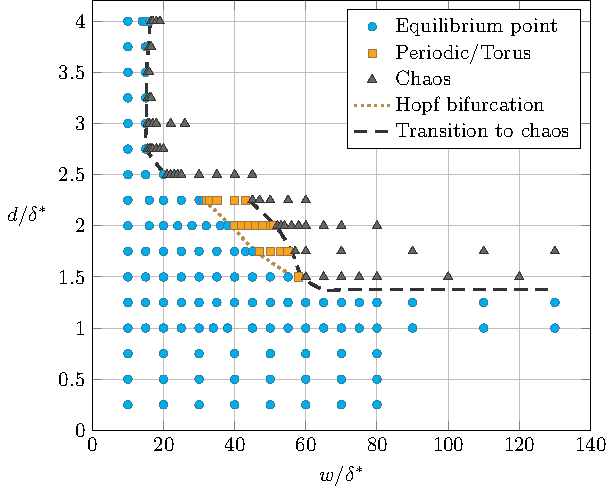
\includegraphics[width=0.6\textwidth]{../../Images/incNS2dStabilityCurve.pdf}
	\caption{Stability diagram showing the dynamical regimes for different gap configurations at $\Rey_dstar =1000$. Gap width $w$ is shown along the horizontal axis and gap depth $d$ along the vertical axis. Blue circles denote steady solutions (equilibria), orange squares represent time-periodic attractors, and black triangles indicate chaotic or turbulent states. The dotted orange line indicate a qualitative boundary for the first Hopf bifurcation while the dashed black line indicate the transition to chaos.}
	\label{fig:stability}
\end{figure}
Blue markers indicate equilibrium solutions of the Navier--Stokes equations, i.e., steady states to which the system converges. As expected, small gaps (either in width or depth) yield stable flows resembling those over a flat plate, corresponding to the limiting cases $w \to 0$ or $d \to 0$.

The internal flow topology within the gap varies with its geometry. Outside the gap, the boundary layer retains a Blasius-like structure. Inside the gap, however, the behavior depends significantly on the available space. Representative steady-state solutions for three different configurations are shown in~\cref{fig:stableSS}. Contours of the wall-normal velocity are displayed along with streamlines to visualize the internal flow structure.

\begin{figure}[ht]
	\centering
	\begin{subfigure}[b]{0.49\textwidth}
		\centering
		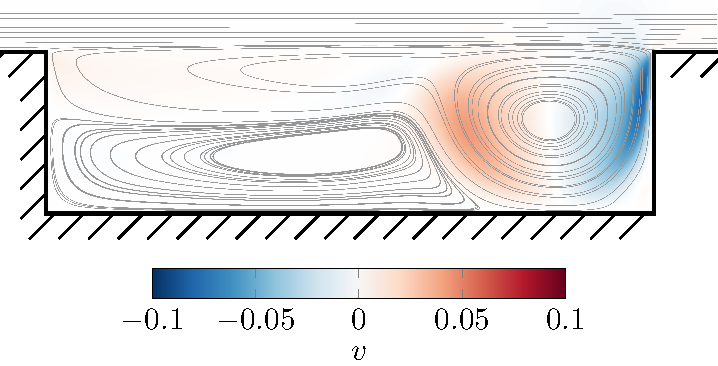
\includegraphics[width=\textwidth]{../../Images/gapd4_w15.pdf}
		\caption{Gap with $w=15\dstar$ and $d=4\dstar$.}
		\label{fig:gapd4w15}
	\end{subfigure}\\[0.5cm]
	\begin{subfigure}[b]{0.49\textwidth}
		\centering
		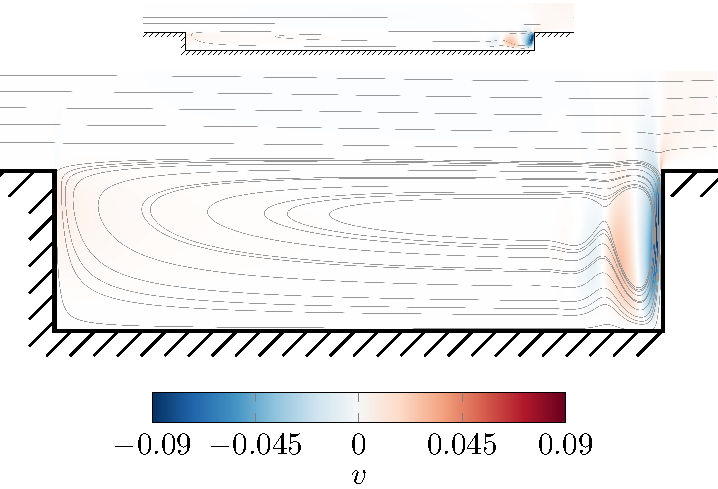
\includegraphics[width=\textwidth]{../../Images/gapd1.5_w30.pdf}
		\caption{Gap with $w=30\dstar$ and $d=1.5\dstar$.}
		\label{fig:gapd15w30}
	\end{subfigure}
	\hfill
	\begin{subfigure}[b]{0.49\textwidth}
		\centering
		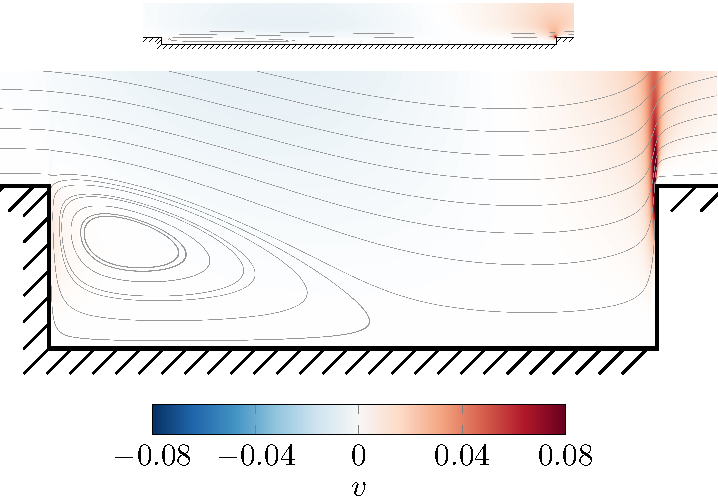
\includegraphics[width=\textwidth]{../../Images/gapd1_w60.pdf}
		\caption{Gap with $w=60\dstar$ and $d=1\dstar$.}
		\label{fig:gapd1w60}
	\end{subfigure}
	\caption{Steady-state flow over three different gap configurations. Wall-normal velocity contours and streamlines are shown in each case. All geometries are rescaled to match the size of the first configuration ($w/d = 15/4$) for visual comparison. The original, unscaled geometries are displayed above the last two cases for reference.}
	\label{fig:stableSS}
\end{figure}

The configurations illustrated in~\cref{fig:stableSS} correspond to $(w/\dstar, d/\dstar) \in \{(15,4), (30,1.5), (60,1)\}$. We observe that for deep gaps, a prominent recirculating region forms near the downstream edge of the cavity. In contrast, shallow gaps do not accommodate such structures; the flow instead enters and exits the cavity more smoothly, exhibiting a weak recirculation zone near the upstream edge.

For fixed gap depth, increasing the width induces a sequence of bifurcations. When the width surpasses a critical threshold that depends on the depth, the flow becomes unstable. For deep gaps ($d/\dstar \in [2.5, 4]$), this transition occurs abruptly, while shallower configurations ($d/\dstar \in [1.5, 2.25]$) exhibit a linearly unstable regime. In this latter region, a Hopf bifurcation emerges, introducing one unstable frequency. A second frequency appears soon after, producing quasiperiodic dynamics on a two-dimensional attracting torus. Spatially, this corresponds to an unstable global mode whose amplitude is concentrated near the downstream edge of the gap, as illustrated in~\cref{fig:absoluteInstability}.

\begin{figure}[H]
	\centering
	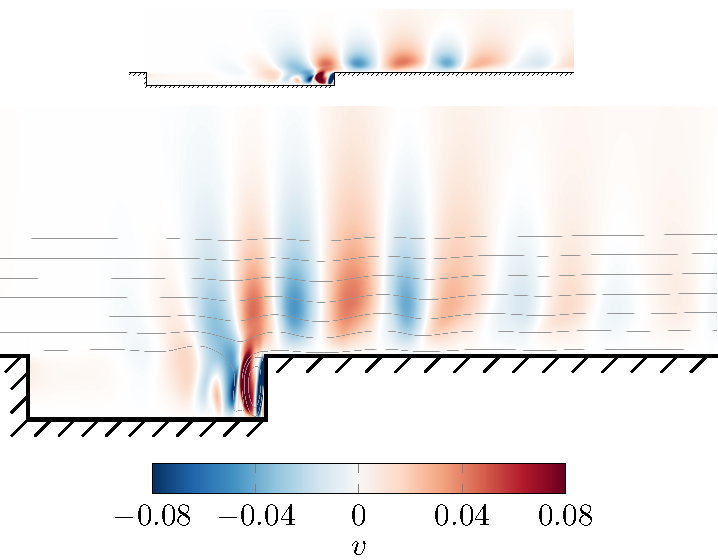
\includegraphics[width=0.49\textwidth]{../../Images/gapd2.25_w35.pdf}
	\caption{Self-sustained absolute instability near the downstream edge of a gap with $w=35\dstar$ and $d=2.25\dstar$. Wall-normal velocity contours are shown. The geometry is rescaled to $w/d=15/4$. The original shape is shown above for reference.}
	\label{fig:absoluteInstability}
\end{figure}

As the width increases further, the attracting torus becomes increasingly distorted. Additional frequencies become less stable, leading ultimately to a chaotic regime~\cite{natureTurbulence}.

\subsection{\texorpdfstring{$\Delta n$}{dn} factors comparison}
\label{sec:results:comparison}

Based on the DNS results, we identify several steady baseflows $\vf{U}$ that serve as a foundation for linear stability analysis (see~\cref{eq:linearizedns}). Using each base flow, we solve the linearized Navier--Stokes equations given in~\cref{eq:linearizedns}. The numerical setup used for this analysis differs from the previous simulations. Since the baseflow already satisfies the boundary conditions, we impose homogeneous boundary conditions of the same type as before. To excite Tollmien--Schlichting (TS) waves, a small perturbation in the wall-normal velocity is introduced at the upstream region of the boundary layer. This perturbation is modeled as white Gaussian noise. Specifically, the wall-normal velocity component is defined as  
\begin{equation}
v(x,t) = A \exp{-w(x-x_0)^2} X_t
\end{equation}
where $A = 0.01$, $w = 5$, $x_0 = -95\delta^*$, and $X_t$ represents a unit-variance white Gaussian noise process. The Gaussian function with the specific weight chosen localizes the excitation to a region of approximately $2\delta^*$ in length, centered at $x_0$. While real experimental disturbances are neither white nor Gaussian, this idealized model is commonly employed for its simplicity and general applicability.


\begin{figure}[ht]
	\centering
	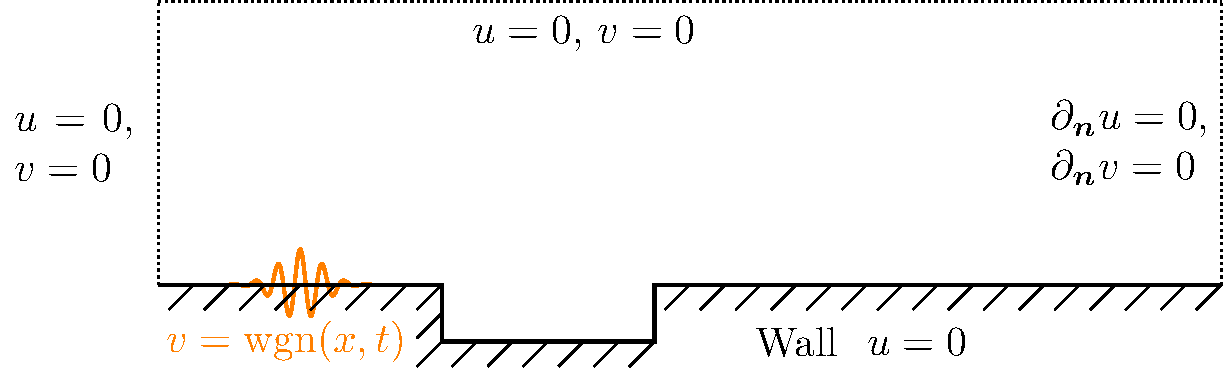
\includegraphics[width=0.75\textwidth]{../../Images/domainPert.pdf}
	\caption{Schematic of the domain used in the stability analysis. White Gaussian noise is introduced in a small band at the upstream region to excite TS waves.}
	\label{fig:pertdomain}
\end{figure}
Since the perturbation is random, so is its amplitude. Therefore, before computing the maximum in~\cref{eq:amplitudeNorm}, we use a time-averaged quantity based on the root-mean-square (RMS) of the velocity components:
\begin{equation}
	A(x) = \max_{y \in \mathcal{Y}(x)} \sqrt{ \left\langle u_i(x,y)^2 + v_i(x,y)^2 \right\rangle }.
	\label{eq:amplitudeRMS}
\end{equation}
Here, $(u_i, v_i)$ are the streamwise and wall-normal components of the perturbation velocity at different time instances, and $\langle \cdot \rangle$ denotes the average over time.

After introducing the forcing, the flow requires a short transient period to stabilize. After this period, the relative perturbation amplitude reaches approximately $5 \times 10^{-4}$ in the streamwise component and $5 \times 10^{-2}$ in the wall-normal component. Simulations are run for a sufficient duration to allow temporal averaging over a set of control points, thereby suppressing stochastic fluctuations.

The minimum perturbation amplitude upstream of the gap is identified and used to compute the $n$-factor curve, $n_{\text{wgn}}(x)$, according to~\cref{eq:nfactorAmplitude}. For simplicity, we drop the subscript and refer to this simply as $n(x)$. 
% The computed $n$-factors for several gap configurations with fixed depth $d = 1\dstar$ and varying width $w$ are shown in~\cref{fig:nfactors}.

% \begin{figure}[ht]
% 	\centering
% 	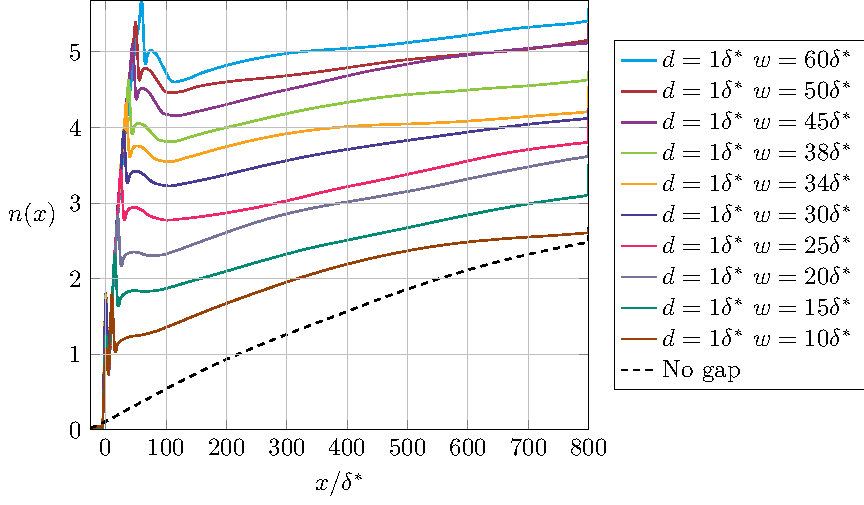
\includegraphics[width=0.8\textwidth]{../../Images/Nfactors.pdf}
% 	\caption{Comparison of $n$-factor curves for various gap configurations with fixed depth $d=1\dstar$ and varying width $w$. The flat-plate reference case is shown as a dashed line.}
% 	\label{fig:nfactors}
% \end{figure}
% We observe that wider gaps lead to greater amplification of TS waves. However, noticeable oscillations appear in the $n(x)$ curves for the gapped cases. These may arise from several main sources. First, the inherent randomness of the perturbation may not have been fully averaged out. Second, the control points used for monitoring were placed at a fixed wall-normal distance of $1\dstar$, even though the boundary layer thickness grows as $\propto\sqrt{x}$. This inconsistency can affect amplification measurements, as discussed in~\cite{bertolotti}. In the framework of LST, the choice of an $L^\infty$ norm for the $y$-dependent amplitude has been shown to provide robust results~\cite{vanVooren}.

To compare with the experimental data of Crouch et al.~\cite{jeffGaps}, we compute the difference between the $n$-factor of each gapped configuration and that of the flat-plate reference case. Since this difference depends on the streamwise coordinate $x$, and our primary interest lies in the amplification of TS waves induced by the gap itself rather than its downstream evolution, we focus on a region of length $100\dstar$ located after the onset of monotonic growth in the $n$-factor curves. We then average the $n$-factors over this interval to obtain a representative amplification value. This difference is denoted by $\Delta n$, rather than $\Delta N$ as in some experimental studies~\cite{jeffGaps,jeffConference}, to emphasize that we are comparing specific growth histories rather than optimal envelope values.

\begin{figure}[ht]
	\centering
	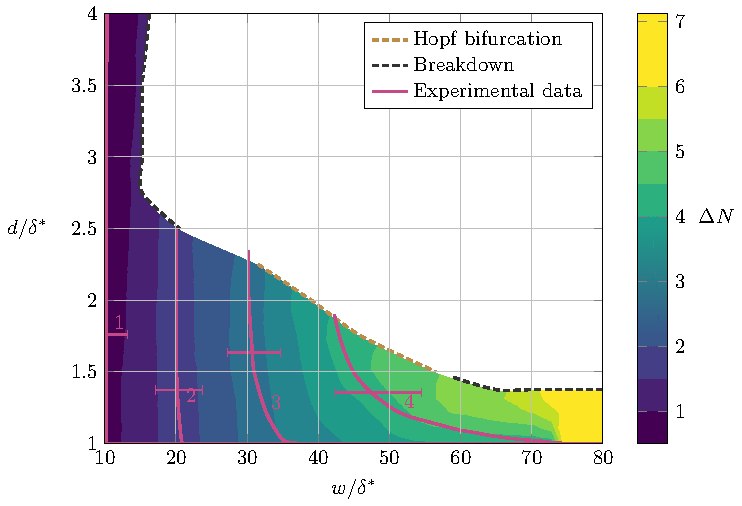
\includegraphics[width=0.7\textwidth]{../../Images/nfactor_countour.pdf}
	\caption{Contour plot of $\Delta n$ factors on the stable side of the parameter grid $(w/\dstar,d/\dstar)\in[0,70]\times[0,4]$. Magenta contours show experimental level lines from~\cite{jeffGaps} for levels 1, 2, 3, and 4.}
	\label{fig:nfactorcountour}
\end{figure}

The $\Delta n$ values are computed at all gap configurations for which a steady baseflow was available. Interpolation is performed inside the convex hull of these points using linear interpolation, while nearest-neighbor extrapolation is applied outside the convex hull, but inside the globally stable region. To reduce artifacts from interpolation noise and the irregularities in the $n(x)$ curves, a Gaussian filter with $\sigma = 0.7$ is applied.

Overall, the comparison with experimental data (see~\cref{fig:nfactorcountour}) shows very good agreement. In particular, we correctly capture both asymptotic regimes: the vertical trend at narrow gaps and the horizontal trend at shallow gaps. We truncate the domain at $w = 70\dstar$, since the amplification becomes large enough to invalidate the linearized Navier--Stokes approximation. Furthermore, simulations in the region $(w/\dstar,d/\dstar)\in[70,140]\times[0,1.25]$ were not extensively performed due to strict numerical stability constraints in the CFL number (see~\cref{fig:stability}). For such cases where $\Delta n$ is higher than 6, nonlinear effects would start becoming important, requiring a fully nonlinear perturbed boundary layer analysis to accurately capture saturation and transition mechanisms.

\end{document}
